\section{Auswertung}
\label{sec:Auswertung}
\subsection{Winkelrichtgröße und Eigenträgheitsmoment}
\begin{table}
    \centering
    \csvreader[tabular=c|c|c,
    head=false,
    table head= $\varphi/\si{\degree}$ & $F/\si{\newton}$ & $D/\si{\newton\metre}$\\
    \midrule,
    late after line= \\]
    {content/data/stange_D.csv}{1=\eins, 2=\zwei, 3=\drei}{$\num{\eins}$ & $\num{\zwei}$ & $\num{\drei}$}
    \caption{Die gemessene Kraft $F$ bei einem Auslenkwinkel $\varphi$ und die daraus resultierende Winkelrichtgröße $D$.}
    \label{tab:kraft}  
\end{table}

\begin{table}
    \centering
    \csvreader[tabular=c|c,
    head=false,
    table head= $a/\si{\centi\metre}$ & $T/\si{\hertz}$ \\
    \midrule,
    late after line= \\]
    {content/data/gewichte.csv}{1=\eins, 2=\zwei}{$\num{\eins}$ & $\num{\zwei}$}
    \caption{Die Schwingungsdauer $T$ bei variablem Abstand $r$ zur Drehachse.}
    \label{tab:gewichte}  
\end{table}
\begin{figure}
    \centering
    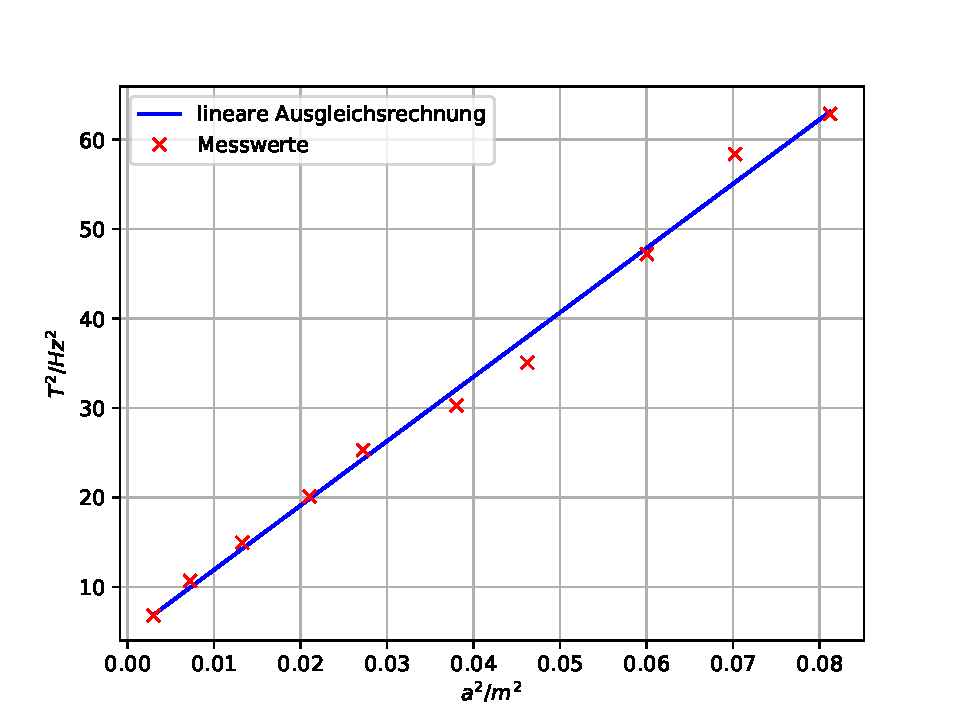
\includegraphics[width=\textwidth]{content/data/ausgleich.pdf}
    \caption{Lineare Ausgleichsrechnung um Eigenträgheitsmoment $I_\text{d}$ zu ermitteln.}
    \label{fig:ausgleich}
\end{figure}
\FloatBarrier

\subsection{Trägheitsmoment eines großen Zylinders}
\begin{table}
    \centering
    \csvreader[tabular=c|c,
    head=false,
    table head= Messung & $T/\si{\second}$ \\
    \midrule,
    late after line= \\]
    {content/data/zylinder_gr.csv}{1=\eins, 2=\zwei}{$\num{\eins}$ & $\num{\zwei}$}
    \caption{Mehrfache Messung der Schwingungsdauer $T$ für den großen Zylinder.}
    \label{tab:zylinder_gr}  
\end{table}
\FloatBarrier

\subsection{Trägheitsmoment eines kleinen Zylinders}
\begin{table}
    \centering
    \csvreader[tabular=c|c,
    head=false,
    table head= Messung & $T/\si{\second}$ \\
    \midrule,
    late after line= \\]
    {content/data/zylinder_kl.csv}{1=\eins, 2=\zwei}{$\num{\eins}$ & $\num{\zwei}$}
    \caption{Mehrfache Messung der Schwingungsdauer $T$ für den kleinen Zylinder.}
    \label{tab:zylinder_kl}  
\end{table}
\FloatBarrier

\subsection{Trägheitsmomente der Modellpuppe}
\subsubsection{Position 1}
\begin{table}
    \centering
    \csvreader[tabular=c|c,
    head=false,
    table head= Messung & $T/\si{\second}$ \\
    \midrule,
    late after line= \\]
    {content/data/modellpuppe1.csv}{1=\eins, 2=\zwei}{$\num{\eins}$ & $\num{\zwei}$}
    \caption{Mehrfache Messung der Schwingungsdauer $T$ für die Modellpuppe in Position 1.}
    \label{tab:modellpuppe1}  
\end{table}
\FloatBarrier

\subsubsection{Position 2}
\begin{table}
    \centering
    \csvreader[tabular=c|c,
    head=false,
    table head= Messung & $T/\si{\second}$ \\
    \midrule,
    late after line= \\]
    {content/data/modellpuppe2.csv}{1=\eins, 2=\zwei}{$\num{\eins}$ & $\num{\zwei}$}
    \caption{Mehrfache Messung der Schwingungsdauer $T$ für die Modellpuppe in Position 2.}
    \label{tab:modellpuppe2}  
\end{table}
\FloatBarrier